\documentclass[a4paper,11pt]{scrartcl}
\usepackage[a4paper, left=2cm, right=2cm, top=2cm, bottom=2cm]{geometry} % kleinere Ränder

%Paket für Header in Koma-Klassen (scrartcl, scrrprt, scrbook, scrlttr2)
\usepackage[headsepline]{scrlayer-scrpage}
% Header groß genug für 3 Zeilen machen
\setlength{\headheight}{3\baselineskip}


% Default Header löschen
\pagestyle{scrheadings}
\clearpairofpagestyles

% nicht kursiv gedruckte header
\setkomafont{pagehead}{\sffamily\upshape}

% Links im Dokuement sowie \url schön machen
\usepackage[colorlinks,pdfpagelabels,pdfstartview = FitH, bookmarksopen = true,bookmarksnumbered = true, linkcolor = black, plainpages = false, hypertexnames = false, citecolor = black]{hyperref}

% Umlaute in der Datei erlauben, auf deutsch umstellen
\usepackage[utf8]{inputenc}
\usepackage[ngerman]{babel}

% Mathesymbole und Ähnliches
\usepackage{amsmath}
\usepackage{mathtools}
\usepackage{amssymb}
\usepackage{microtype}
\newcommand{\NN}{{\mathbb N}}
\newcommand{\RR}{{\mathbb R}}
\newcommand{\QQ}{{\mathbb Q}}
\newcommand{\ZZ}{{\mathbb{Z}}}

% Komplexitätsklassen
\newcommand{\pc}{\ensuremath{{\sf P}}}
\newcommand{\np}{\ensuremath{{\sf NP}}}
\newcommand{\npc}{\ensuremath{{\sf NPC}}}
\newcommand{\pspace}{\ensuremath{{\sf PSPACE}}}
\newcommand{\exptime}{\ensuremath{{\sf EXPTIME}}}
\newcommand{\CClassNP}{\textup{NP}\xspace}
\newcommand{\CClassP}{\textup{P}\xspace}

% Weitere pakete
\usepackage{multicol}
\usepackage{booktabs}

% Abbildungen
\usepackage{tikz}
\usetikzlibrary{arrows,calc}

% Meistens ist \varphi schöner als \phi, genauso bei \theta
\renewcommand{\phi}{\varphi}
\renewcommand{\theta}{\vartheta}

% Aufzählungen anpassen (alternativ: \arabic, \alph)
\renewcommand{\labelenumi}{(\roman{enumi})}



% Header i-> inner (bei einseitig links), c -> center, o -> Outer (bei einseitg rechts)
\ihead{Model Checking\\
	SoSe 2022 \\\today}
\chead{\Large Exercise Sheet 1}
\ohead{Peter Reithofer, 394407 \\
	   László Dirks, 398777 \\
	   Khulan Bayarkhuu, 394604}

	
\cfoot*{\pagemark} % Seitenzahlen unten

\begin{document}
	
	\section*{Exercise 1 (Open a Bank Account)}
	Our friend performs tests for a few initial inputs. The input values seem to be chosen to cover edge cases regarding the amount of the initial deposit. However this does not deal with what happens with the deposit once it has been accepted to have a valid initial amount.
	
	In Line 2 of Algorithm 1 the user is free to "do something" with the deposit. This could mean that the user withdraws more than they deposited, leading to a negative balance. This case would not necessarily be detected by simply testing various initial inputs as it further depends on the possible actions of the user. 
	
	Model checking might allow us to detect such a flaw by reasoning about the entire possible state space and not only a few selected scenarios.
	
	\section*{Exercise 2 (Transition Systems)}
	
	\begin{itemize}
		\item[a)] $ TS_1 = \bigl( \{s_0, s_1, s_2, s_3, s_4\}, \{\alpha,\beta, \gamma\}, \\
		\{ (s_0, \alpha, s_2), (s_0, \gamma, s_1), (s_1, \gamma, s_1), (s_1, \alpha, s_3), (s_1, \beta, s_4), (s_2, \alpha, s_0), (s_2, \beta, s_4), (s_4, \alpha, s_2), (s_4, \gamma, s_3)\},\\
		\{s_0\}, \bigl\{ \{a\}, \{b\}, \{a,b\} \bigr\}, L_1 \bigr)$\\
		with $L_1: \bigl\{ \{s_0 \mapsto \{a\}, s_1 \mapsto \{a\}, s_2 \mapsto \{a,b\}, s_3 \mapsto \{b\}, s_4 \mapsto \{a,b\} \bigr\}$.
		\item[b)] Here is an example for a finite execution: $\rho_{finite} = s_0 \gamma s_1 \alpha s_3$ and an example for an infinite execution: $\rho_{infinite} = s_0 \gamma s_1 \gamma s_1 \gamma s_1 \dots$.
		\item[c)]
		\begin{itemize}
			\item[(i)] $TS_1$ is $AP$-deterministic, because $\mid I \mid = \mid \{s_0\} \mid = 1 \leq 1$ and there are only at most 2 states $s$ and $s'$ for which $L(s)=L(s')$ holds: For these pairs $(s_0, s_1)$ with $L(s_0)=L(s_1)=\{a\}$ and $(s_2, s_4)$ which $L(s_2)=L(s_4)=\{a, b\}$ are never both in $Post(s'')$ for all $s'' \in S$.
			%for the every $A$ for which holds $\{L(s')=A\} > 1$ except for $A \in \bigl\{ \{a\}, \{a,b\} \}$
			
			\item[(ii)] $TS_1$ is also $action-deterministic$, because both conditions hold:
			\begin{itemize}
				\item $\mid I \mid = \mid \{s_0\} \leq 1$
				\item $|Post(s_0, \alpha)| = |Post(s_0, \gamma)| = |Post(s_1, \alpha)| = |Post(s_1, \beta)|= |Post(s_1, \gamma)|= |Post(s_2, \alpha)| = |Post(s_2, \beta)| = |Post(s_4, \alpha)|= |Post(s_4, \gamma)| = 1$ and for every other pair $(s_i, \sigma)$ with $s_i \in \{s_0, s_1, s_2, s_3, s_4\}$ and $\sigma \in \{\alpha, \beta, \gamma\}$ holds $(s_i, \sigma)=0$.
			\end{itemize}
		\end{itemize}
		\item[d)] $ TS_2 = \bigl( \{s_0, s_1, s_2, s_3\}, \{\alpha,\beta, \gamma\}, \\
		\{ (s_0, \alpha, s_2), (s_0, \gamma, s_1), (s_1, \gamma, s_1), (s_1, \alpha, s_3), (s_1, \beta, s_2), (s_2, \alpha, s_0), (s_2, \beta, s_1), (s_3, \beta, s_2), (s_3, \beta, s_3) \}\\
		\{s_0\}, \bigl\{ \{a\}, \{b\}, \{a,b\} \bigr\}, L_2 \bigr)$\\
		with $L_2: \bigl\{ \{s_0 \mapsto \{a\}, s_1 \mapsto \{a\}, s_2 \mapsto \{a,b\}, s_3 \mapsto \{b\}\bigr\}$.
		\item[e)] An example for a path in $TS_2$ is $\pi := (s_0, s_1, s_1, s_1, \dots)$ and therefore $trace(\pi)=\{a\}\{a\}\{a\}\dots$.
		\item[f)]
		\begin{itemize}
			\item[(i)] $TS_2$ is not $AP-deterministic$, because the second condition does not hold: 
			\item[(ii)] 
		\end{itemize}
	\end{itemize}
	
	\section*{Aufgabe 3 (Program Graphs)}
	\begin{itemize}
		\item[a)] \begin{figure}[h]
			\centering
			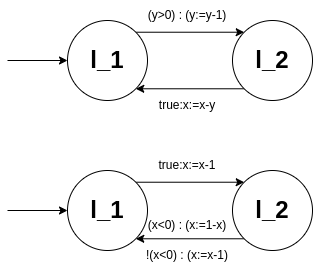
\includegraphics[width=0.5\textwidth]{t3a}
			\caption{}
			\label{fig:t3a}
		\end{figure}
		\item[b)] \begin{figure}[h]
			\centering
			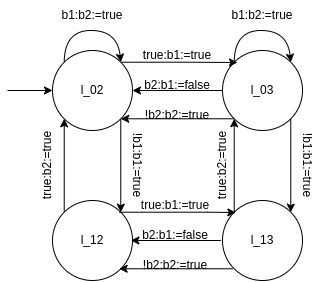
\includegraphics[width=0.5\textwidth]{t3b}
			\caption{}
			\label{fig:t3b}
		\end{figure}
		\item[c)] \begin{figure}[h]
			\centering
			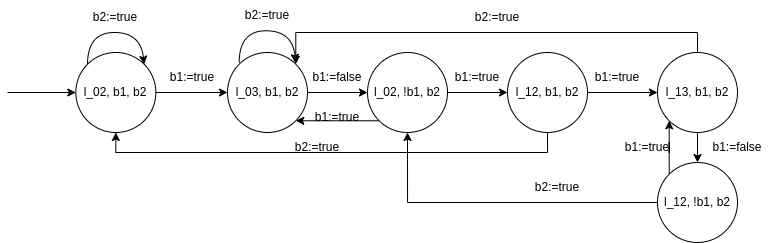
\includegraphics[width=0.5\textwidth]{t3c}
			\caption{}
			\label{fig:t3c}
		\end{figure}
	\end{itemize}

		
	
	\section*{Aufgabe 4 (Handshaking)}
	
	\begin{itemize}
		\item[a)]
		\item[b)]
		\item[c)]
	\end{itemize}
	
\end{document}

